\documentclass[12pt]{article}

\usepackage{blindtext} % Package to generate dummy text throughout this template 

\usepackage[utf8]{inputenc}
\usepackage{amsmath, amssymb}
\usepackage{algorithm}
\usepackage[noend]{algpseudocode}
\linespread{1.25}
\usepackage[margin = 1in]{geometry}
\usepackage{microtype} % Slightly tweak font spacing for aesthetics
\usepackage[english]{babel} % Language hyphenation and typographical rules
\usepackage{tikz}
\usepackage{hyperref}
\usepackage{url}
\usepackage{graphicx}
\usepackage{float}
\usepackage{wrapfig}
\usepackage{subcaption}
\hypersetup{
    colorlinks=true,
    linkcolor=red,      
    urlcolor=blue,
    bookmarks=true,
    citecolor=green!75!black
}

\setlength{\parindent}{2em}
%\setlength{\parskip}{1.5em}
\graphicspath{ {images/} }

\newcommand{\vect}[1]{\mathbf{#1}}  % vector
\newcommand{\matr}[1]{\mathbf{#1}}  % matrix
\newcommand{\tens}[1]{\mathbf{#1}}  % tensor
\newcommand{\mean}[1]{\overline{#1}}    % mean overline
\newcommand\Algphase[1]{%
    \vspace*{-.7\baselineskip}\Statex\hspace*{\dimexpr-\algorithmicindent-2pt\relax}\rule{\textwidth}{0.4pt}%
    \Statex\hspace*{-\algorithmicindent}\textbf{#1}%
    \vspace*{-.5\baselineskip}\Statex\hspace*{\dimexpr-\algorithmicindent-2pt\relax}\rule{\textwidth}{0.4pt}%
}

\begin{document}
    \tableofcontents
    \listoftables
    \listoffigures
    \section{Introduction} \label{sec:Introduction}
    Optimizing predictive models on datasets that are obtained from citizen-science projects can be computationally expensive as these datasets grow in size with time. Consequently, models based on multiple-layered neural networks, Integer Programming and other optimization routines can prove increasingly difficult as the number of parameters increase, despite using the faster Central Processing Units (CPUs) in the market. Incidentally, it becomes difficult for citizen-science projects to scale if the organizers use CPUs to run optimization models. However, Graphical Processing Units (GPUs), which offer multiple cores to parallelize computation, can outperform CPUs in computing such predictive models if these models heavily rely on large-scale matrix multiplications. By using GPUs over CPUs to accelerate computation on a citizen-science project, the model could achieve better optimization in less time, enabling the project to scale.\\
    
    Part of the eBird project, which aims to ``maximize the utility and accessibility of the vast numbers of bird observations made each year by recreational and professional bird watchers'', Avicaching is a incentive-driven game trying to homogenize the spatial distribution of citizens' (agents') observations [cite website]. Since the dataset of agents' observations in eBird is geographically heterogeneous (concentrated in some places like cities and sparse in others), Avicaching homogenizes the observation set by rewarding agents who visit under-sampled locations \cite{Xue2016Avi1}. To accomplish this task of specifying rewards at different locations based on the historical records of observations, Avicaching would learn the change in agents' behavior when a certain sample of rewards were applied to the set of locations, and then distribute a newer set of rewards across the locations based on those learned parameters \cite{Xue2016Avi2}. This requirement naturally translates into a predictive optimization problem, which was implemented using multiple-layered neural networks and linear programming.

    \subsection{Computation Using GPUs} \label{sec:comp_using_GPUs}
    
    \section{Problem Formulation} \label{sec:Problem Formulation}
    Since NVIDIA General Purpose GPUs enable faster computation on matrices, accelerated through CUDA and cuDNN, both the Identification (Section \ref{sec:Identification Problem}) and the Pricing Problem (Section \ref{sec:Pricing Problem}) were formulated as 3-layered neural networks using the PyTorch library.
    
    \subsection{Identification Problem} \label{sec:Identification Problem}
    As discussed in Section \ref{sec:Introduction}, the model would need to learn parameters that caused the change in agents' behavior when a certain set of rewards was applied to locations in the experiment region. Specifically, given datasets $\vect{y_t}$ and $\vect{x_t}$ of agents' visit densities with and without the rewards $\vect{r_t}$, we want to find weights $\matr{w_1}$ and $\matr{w_2}$ that caused the change from $\vect{x_t}$ to $\vect{y_t}$, factoring in possible influence from environmental factors $\matr{f}$ and distances between locations $\matr{D}$. Although the original model proposed to learn a single set of weights $\matr{w}$ \cite{Xue2016Avi2}, this proposed model considers two sets of weights $\matr{w_1}$ and $\matr{w_2}$ as it may theoretically result into higher accuracy and lower loss. Mathematically, our model can be formulated as:
    \begin{equation} \label{eq:iden_problem}
    \begin{aligned}
    & \underset{\matr{w}}{\text{minimize}}
    & & Z_I(\matr{w_1}, \matr{w_2}) = \sum_{t} (\omega(\vect{y_t} - \matr{P}(\matr{f}, \vect{r_t}; \matr{w_1}, \matr{w_2})\vect{x_t}))^{2}
    \end{aligned}
    \end{equation}
    where $\omega$ is a set of weights at time $t$ capturing penalties relative to the importance of homogenizing at different locations and elements $p_{u, v}$ of $\matr{P}$ are given as:
    \begin{equation} \label{eq:puv_equation}
    p_{u, v} = \frac{\exp(\matr{w_2} \cdot \text{reLU} (\matr{w_1} \cdot [d_{u, v}, \vect{f_{u}}, r_{u}]))}{\sum_{u'} \exp(\matr{w_2} \cdot \text{reLU} (\matr{w_1} \cdot [d_{u', v}, \vect{f_{u'}}, r_{u'}]))} = \frac{\exp(\Gamma_{u, v})}{\sum_{u'}\exp(\Gamma_{u', v})} = \text{softmax}(\Gamma_{u, v})
    \end{equation}
    In the expression for $p_{u,v}$ (Equation \ref{eq:puv_equation}), softmax$(\cdot)$ is the function: softmax$(z_i) = \frac{\exp(z_i)}{\sum_{i}\exp(z_i)}$ and the reLU$(\cdot)$ function is a ``rectified Linear Unit'' defined as: reLU$(z) = \text{max}(0, z)$.\\
    To optimize the loss value $Z_I(\matr{w_1}, \matr{w_2})$ (Equation \ref{eq:iden_problem}), the neural network learns the set of weights through multiple iterations of backpropagating the loss using gradient descent. Furthermore, the program would process the dataset before feeding to the network to avoid unnecessary sub-iterations and promote batch operations on matrices. 
    
    \subsubsection{Structure of Input Dataset} \label{sec:Structure of Input Dataset}
    \begin{figure}[H]
        \begin{subfigure}{.64\textwidth}
            \centering
            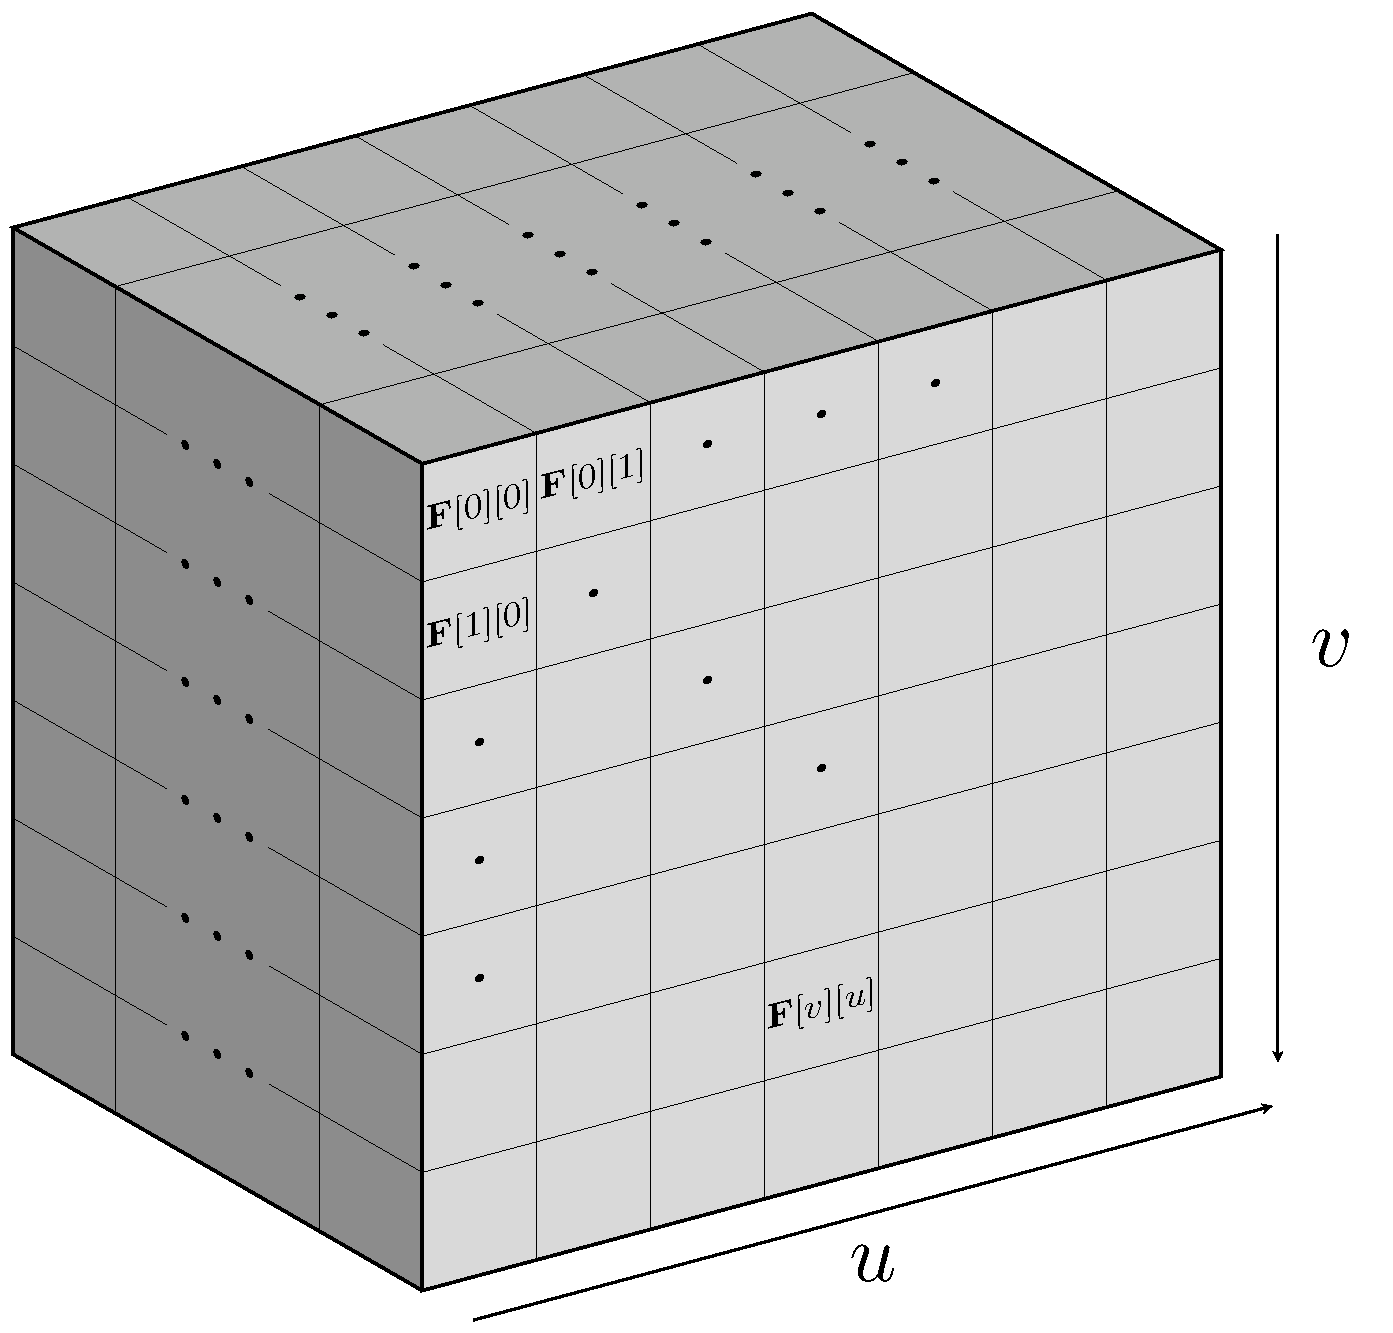
\includegraphics[width=\linewidth]{weights_input_dataset}
            \caption{A Tensor representing the Input Dataset $\matr{F}$}
            \label{fig:A Tensor representing the complete Input Dataset}
        \end{subfigure}
        \begin{subfigure}{.35\textwidth}
            \centering
            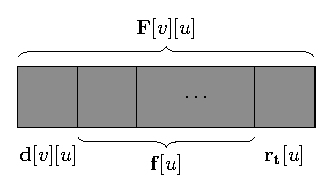
\includegraphics[width=\linewidth]{zoomup_Fuv}
            \caption{Contents of $\matr{F}[v][u]$}
            \label{fig:Zoomed-in contents of Fvu}
        \end{subfigure}
        \caption{Visual representation of the Input Dataset}
        \label{fig:Visual representation of the Input Dataset}
    \end{figure}
    Since preprocessing the dataset impacts the efficiency of the network, the input dataset, comprising of distance between locations $\matr{D}$, environmental features $\vect{f}$ and given rewards $\vect{r_t}$ (all normalized) were combined in a specific manner. Since GPUs are efficient in operating on matrices and tensors, the input dataset was combined into a tensor (Figure \ref{fig:A Tensor representing the complete Input Dataset}) such that batch operations could be performed on slices $\matr{F}[v]$. Another advantage of building the dataset as a tensor comes with the PyTorch library, which provides convenient handling and transfer of tensors residing on CPUs and GPUs. Algorithm \ref{alg:Constructing the Input Dataset} describes the steps to construct this dataset.
    \begin{algorithm}
        \caption{Constructing the Input Dataset} \label{alg:Constructing the Input Dataset}
        \begin{algorithmic}[1]
            \Function{Build-Dataset}{$\matr{D}, \matr{f}, \matr{r_t}$}
            \State $\matr{D} \gets \Call{Normalize}{\matr{D}}$\Comment{$\matr{D}[u][v]$ is the distance between locations $u$ and $v$}
            \State $\vect{f} \gets \Call{Normalize}{\mathbf{f}, axis = 0}$\Comment{$\mathbf{f}[u]$ is a vector of env. features at location $u$}
            \State $\vect{r_t} \gets \Call{Normalize}{\vect{r_t}, axis = 0}$\Comment{$\vect{r_t}[u]$ is the reward at location $u$}
            \For{$v = 1, 2, \dots, J$}
                \For{$u = 1, 2, \dots, J$}
                    \State $\tens{F}[v][u] \gets [\matr{D}[v][u], \vect{f}[u], \vect{r_t}[u]]$ \Comment{As depicted in Figure \ref{fig:Zoomed-in contents of Fvu}}
                 \EndFor
            \EndFor
            \State \Return $\matr{F}$
            \EndFunction
        \end{algorithmic}
    \end{algorithm}
       
    \subsubsection{Algorithm for the Program} \label{sec:Algorithm for the Program}
    As shown in Figure \ref{fig:Neural network designed for the Identification Problem}, the neural network was made of 3 fully connected layers - the input layer, the hidden layer with rectified Linear Units (reLU), and the output layer generating the results using the softmax$(\cdot)$ function. The network can also be visualized as a collection of 1-dimensional layers (Figure \ref{fig:Side view of the network}), with the softmax$(\cdot)$ calculated on the collection's output.
    \begin{figure}[H]
        \begin{subfigure}{.64\textwidth}
        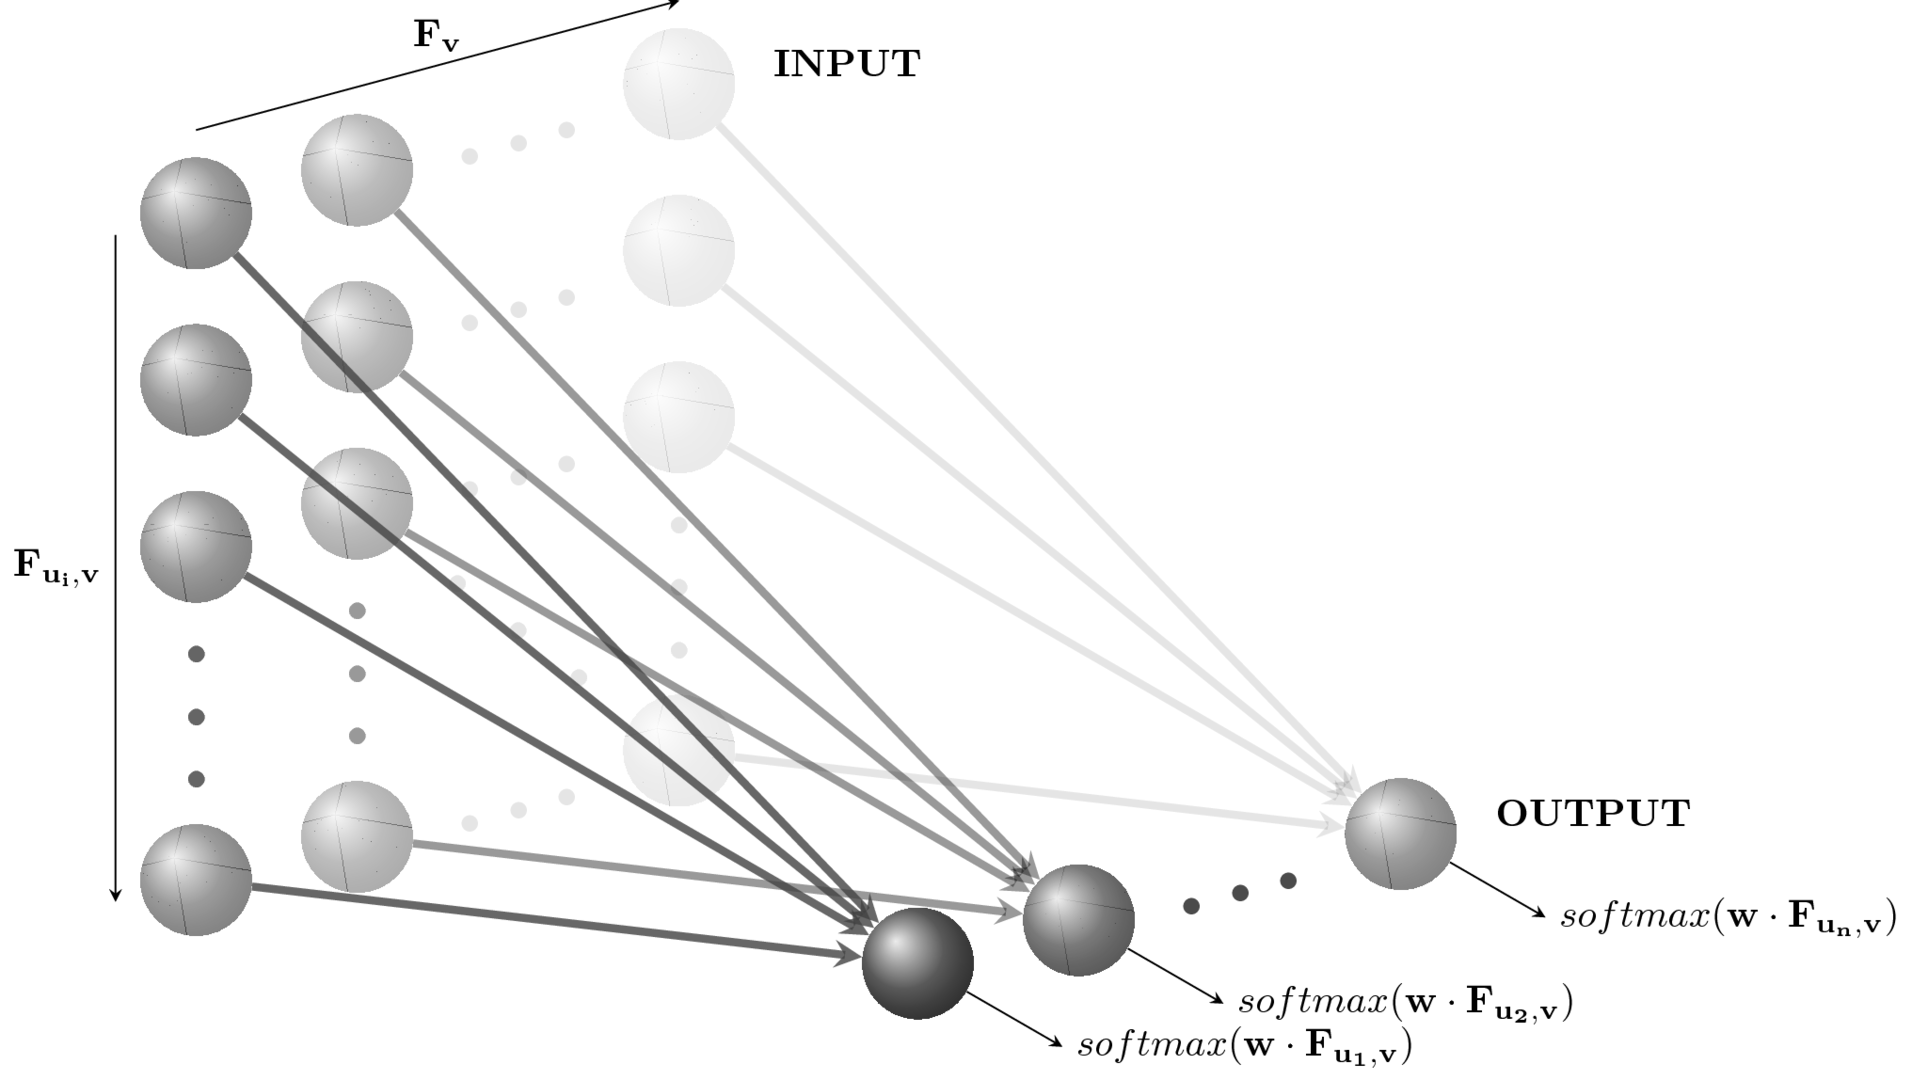
\includegraphics[width=\textwidth]{weights_net}
        \caption{3-dimensional view of the network slice, taking in $\matr{F}[v]$}
        \label{fig:3-dimensional view of the network slice, taking in Fv}
        \end{subfigure}
        \begin{subfigure}{.35\textwidth}
            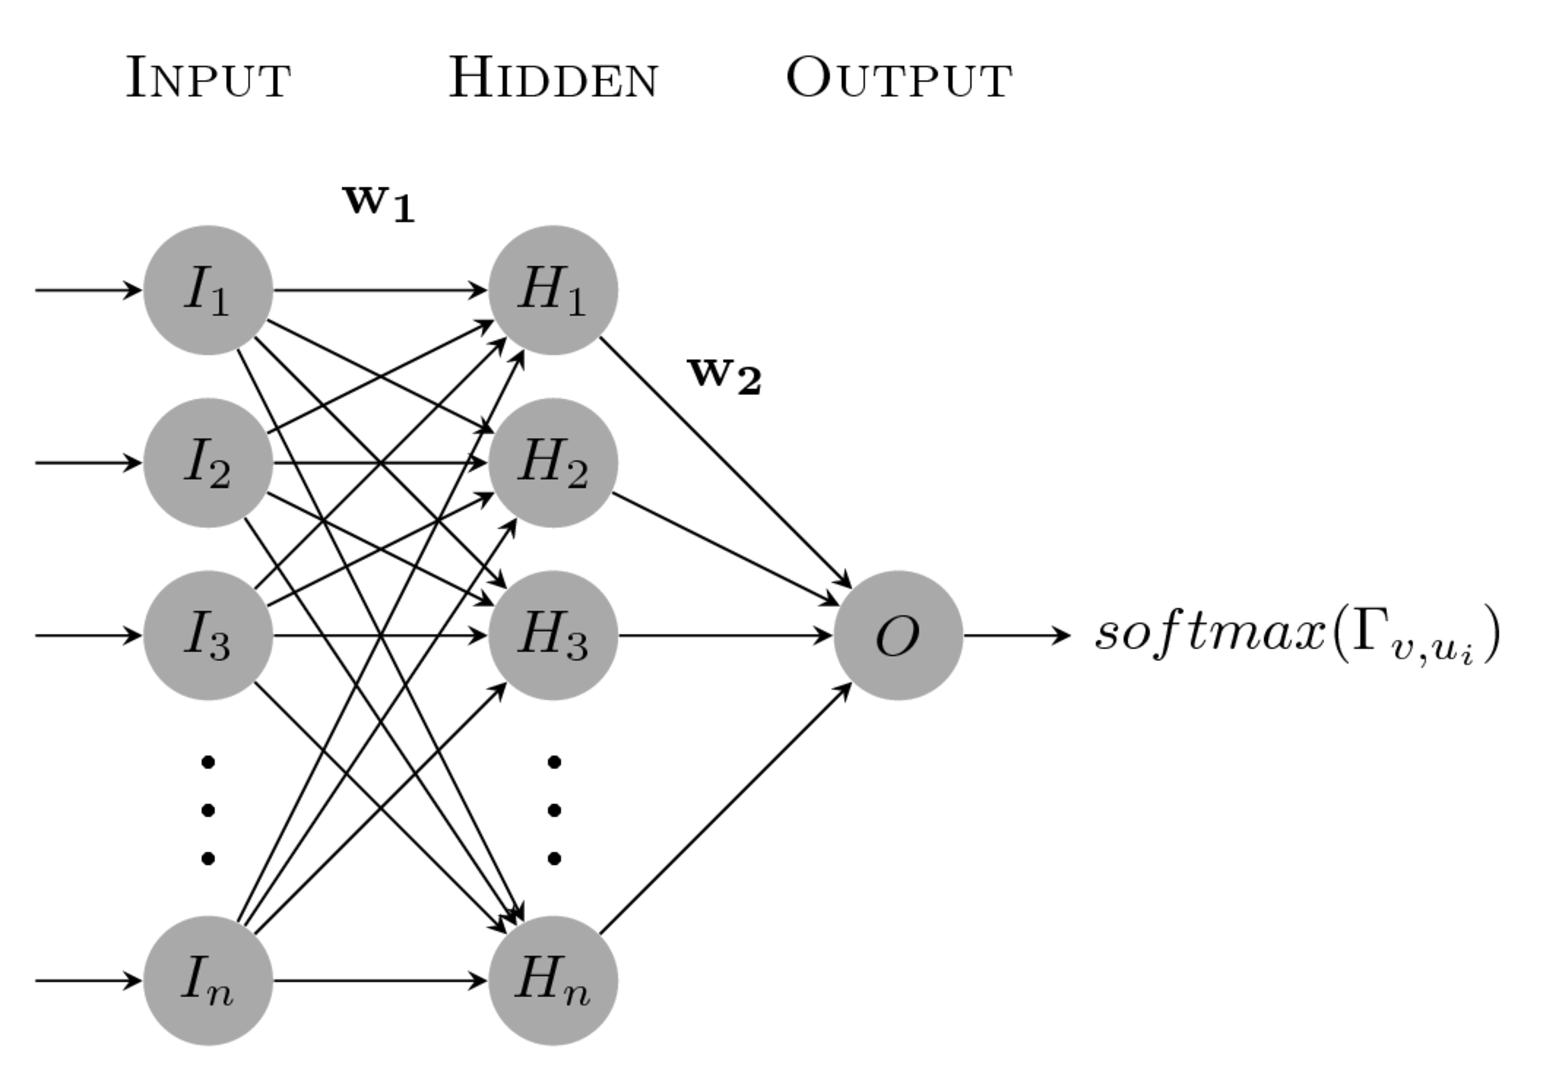
\includegraphics[width=\textwidth]{weights_net_side}
            \caption{Side view of the network}
            \label{fig:Side view of the network}
        \end{subfigure}
        \caption{Neural network designed for the Identification Problem}
        \label{fig:Neural network designed for the Identification Problem}
    \end{figure}
    It is important to clarify that the network in Figure \ref{fig:3-dimensional view of the network slice, taking in Fv}, which takes in $\matr{F}[v]$ as shown, is a slice of the original network, which takes in the complete tensor $\matr{F}$ and computes the complete result $\matr{P}^{T}$  per iteration of $t$. Algorithm \ref{alg:Algorithm for the Identification Problem per iteration} details the steps for learning the parameters $\matr{w_1}$ and $\matr{w_2}$.
    \begin{algorithm}
        \caption{Algorithm for the Identification Problem per iteration} \label{alg:Algorithm for the Identification Problem per iteration}
        \begin{algorithmic}[1]
            \Function{Identify-Weights}{$\matr{x}, \matr{y}, \matr{r}, \matr{D}, \matr{f}, \omega$}
            \For{$t = 1, 2, \dots, T$}
                \State $\matr{F} \gets \Call{Build-Dataset}{\matr{D}, \matr{f}, \matr{r}[t]}$\Comment{Defined in Algorithm \ref{alg:Constructing the Input Dataset}}
                \State $\matr{\Lambda} \gets \text{reLU}(\Call{Batch-Multiply}{\matr{F}, \matr{w_1}})$\Comment{\textbf{Phase 1: Feed Forward}}
                \State $\matr{\Gamma} \gets \text{softmax}(\Call{Batch-Multiply}{\matr{\Lambda}, \matr{w_2}})$
                \State $\matr{P} \gets \matr{\Gamma}^T$
                \State $loss \gets loss + (\omega(\matr{y}[t] - \matr{P} \cdot \matr{x}[t]))^2$
            \EndFor
            \State $\Call{Gradient-Descent}{loss, \matr{w_1}, \matr{w_2}}$\Comment{\textbf{Phase 2: Backpropagate \& Update}}
            \State $\matr{w_1}, \matr{w_2} \gets \Call{Update-Weights}{\matr{w_1}, \matr{w_2}}$
            \EndFunction
        \end{algorithmic}
    \end{algorithm}

    \subsection{Pricing Problem} \label{sec:Pricing Problem}
    After learning the set of weights $\matr{w_1}$ and $\matr{w_2}$ highlighting the change in agents' behavior to collect observations, the Pricing Problem would redistribute rewards to the all locations such that the predicted behavior of agents influenced by the new set of rewards is homogeneous. Thus, given a budget of rewards $\mathcal{R}$, this optimization problem can be expressed as:
    \begin{equation} \label{eq:pricing_problem}
    \begin{aligned}
    & \underset{\vect{r}}{\text{minimize}}
    & & Z_P(\vect{r}) = \frac{1}{n}\lVert \vect{y} - \mean{\vect{y}} \rVert\\
    & \text{subject to}
    & & \vect{y} = \matr{P}(\matr{f}, \vect{r}; \matr{w_1}, \matr{w_2}) \, \vect{x}\\
    &&& \sum_{i} r_i \leq \mathcal{R}\\
    &&& r_i \geq 0
    \end{aligned}
    \end{equation}
    where elements of $\matr{P}$ are defined as in Equation \ref{eq:puv_equation}. 
    
    \section{Experiments}
    
    \section{Results}
    \section{Conclusion}
    
    \blindtext
    \bibliographystyle{ieeetr}
    \bibliography{avicaching}
\end{document}